\chapter{Fundamentação Teórica}\label{cap:fundament}



Esse capítulo tem como objetivo apresentar conceitos que facilitarão o entendimento do conteúdo do capítulo \ref{cap:solucao}, detalhando técnicas e conceitos utilizados na execução do trabalho através de exemplos e imagens. Serão apresentados conceitos relacionados ao processamento de imagens estáticas, seguidos de uma discussão breve sobre técnias aplicadas em vídeos. Por fim serão detalhados as redes neurais e o conceito de classificação de padrões.

\section{Processamento de Imagens}\label{sec:processamento}

\subsection{Imagens em nível de cinza}

Para que um computador seja capaz de operar sobre uma imagem, é preciso que seja utilizado um modelo de representação que traduza o que os nossos sentidos conseguem perceber em informações que podem ser interpretadas por uma máquina que não é dotada de visão. A forma mais simples de se representar uma imagem são as imagens em nível de cinza. Podemos definir imagens como uma função \textit{f{x,y}} onde x e y são coordenadas espaciais e o valor de  \textit{f{x,y}} é a luminosidade, ou nível de cinza, da imagem naquele ponto. Quando esses valores são todos discretos, chamamos essa imagem de uma imagem digital.\cite{gonzalez2009digital} Cada elemento individual dessa imagem, cada valor em cada coordenada, pode ser chamado de um \textit{picture element} ou mais comumente \textit{pixel}. Em imagens digitais em nível de cinza, cada \textit{pixel} possui 1 \textit{bit} de informação, ou seja, pode assumir valores entre 0 e 255, onde o valor 0 representa o preto e 255 representa o branco. 

Uma imagem então, pode ser interpretada por um programa de computador como uma matriz $MxN$ de elementos de 1 \textit{bit}, onde M é a largura da imagem e N é a sua altura. Cada elemento $p_{i,j}$ da matriz possui a informação de luminosidade do pixel correspondente e o computador é capaz de exibir e interpretar esses valores apropriadamente. A figura \ref{fig:NivelCinza} exemplifica esse processo.

\begin{figure}
 \centering
\begin{subfigure}{.5\textwidth}
  \centering
  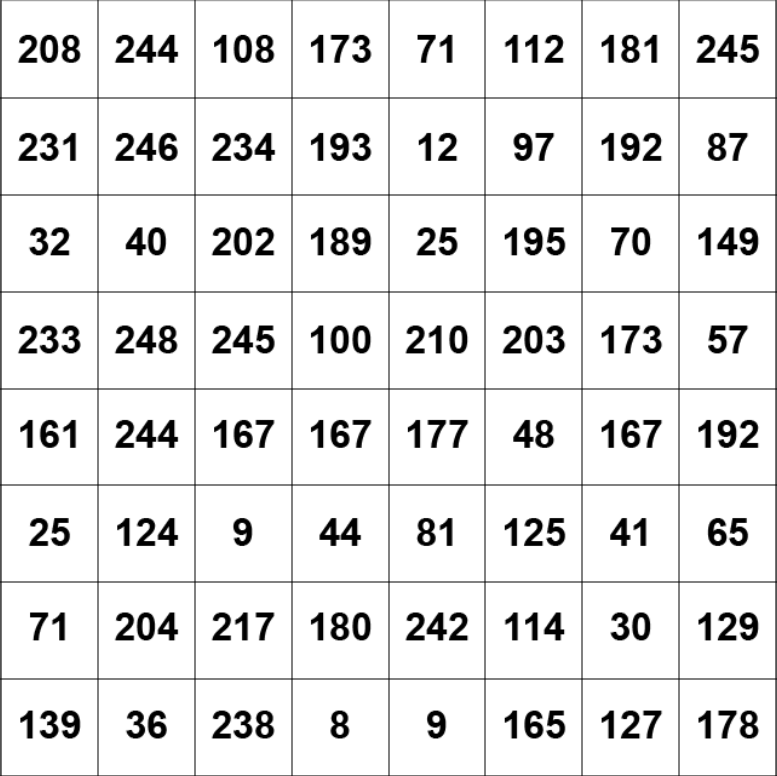
\includegraphics[width=.5\linewidth]{MatrizNivelCinza}
  \caption{}
  \label{exemplo:sfig1}
\end{subfigure}%
\begin{subfigure}{.5\textwidth}
  \centering
  
\includegraphics[width=.5\linewidth]{ExemploNivelCinza}
  \caption{}
  \label{exemplo:sfig2}
\end{subfigure}
\caption{(a) Uma matriz com níveis de cinza e (b) a imagem correspondente}
\label{fig:NivelCinza}
\end{figure}


\subsection{Espaços de cores}

Para que um sistema de processamento de imagens possa interpretar e processar cores, é preciso criar modelos apropriados para representá-las. Chamamos os modelos de representação das cores em uma imagem um espaços de cor. Existem diversos espaços de cor, cada um importante para a realisação de tarefas e necessidades diferentes. Para a compreensão deste trabalho, é necessário, porém, entender apenas dois: o espaço RGB e o espaço YCbCr.

\subsection{O espaço RGB}


RGB é um acrônimo para \textit{Red, Green, Blue}, vermelho, verde e azul em inglês. Pesquisas mostram que um grande gama de cores pode ser formado através de combinações aditivas das cores vermelho, verde e azul. Essas cores são consideradas então cores primárias aditivas.\cite{IBGE2000introducao}. Nesse modelo, a cor de um \textit{pixel} de uma imagem é representada através de um três coeficientes que definem a influência de cada cor primária na combinação. Uma imagem no modelo RGB é então representada por três matrizes de níveis de cinza de dimensões iguais, chamadas canais, onde cada valor representado na matriz, representa o valor do coeficiente da cor correspondente na imagem final. Isto é, a imagem pode ser representada por uma matriz $MxNx3$ onde a cor final $C_{i,j}$ de cada \textit{pixel} da imagem é definida pela equação \ref{eq:corRGB}. A imagem \ref{fig:Espacos:sub:RGB} mostra os canais de uma imagem RGB separadamente.

Esse espaço de cor é o mais comumente encontrado no cotidiano, uma vez que é semelhante visão humana e portanto é utilizado pelos dispositivos multimídia mais comuns.
	
	\begin{equation}\label{eq:corRGB}
			C_{i,j} = p_{i,j,1} . R + p_{i,j,2} . G + p_{i,j,3} . B ,  (0<i<M, 0<j<N)
	\end{equation}

\subsection{Espaço YCbCr}

Assim como o espaço de cor RGB, o espaço YCbCr também representa uma imagem através de três matrizes, porém, seus canais contém informações diferentes do modelo RGB. Esse modelo, é muito utilizado para o armazenamento de vídeos, uma vez que o modelo tira vantagem de alguns aspectos da visão humana para poder armazenar menos dados, sem perda significativa de informação visual. Por exemplo, humanos são mais sensíveis à detalhes e variações em níveis de cinza do que detalhes em imagens coloridas. Além disso, o olho humano é mais sensível ao verde do que qualquer outra cor\cite{colorSpacesDigitalVideo}. Com esse conhecimento, o espaço YCbCr representa as cores de uma imagem através de sua luminosidade(Y) e os valores de crominância azul(Cb) e crominância vermelha(Cr). Cb e Cr são sinais de diferença de cor e são definidos pela subtração do valor de luminosidade do canal azul e vermelho da imagem, respectivamente. A luminosidade é definida pela equação \ref{eq:Y}\cite{LivroVideoDigital} que reflete a sensibilidade maior a cor verde da visão humana.

Na figura \ref{fig:Espacos:sub:YCbCr} estão exemplificados os canais de uma imagem no espaço YCbCr.

\begin{equation}\label{eq:Y}
	Y = 0,299.R + 0,587.G + 0,114.B

\end{equation}


\begin{figure}
 \centering
\begin{subfigure}{.5\textwidth}
  \centering
  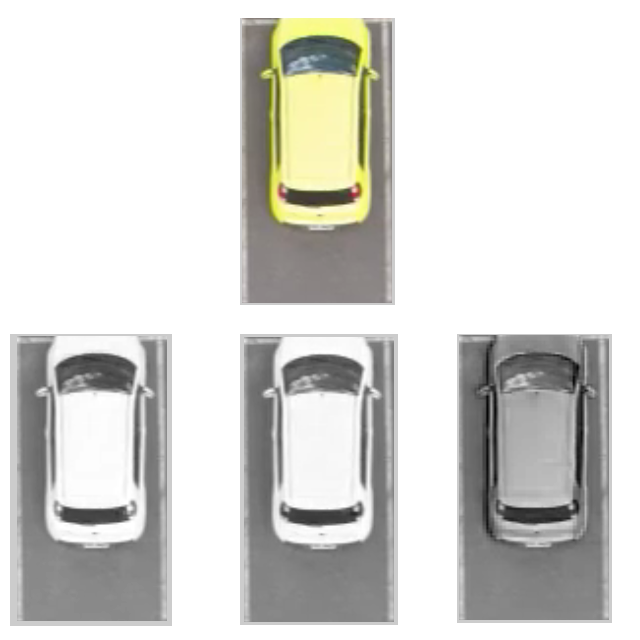
\includegraphics[width=.8\linewidth]{exemploRGBFinal}
	\caption{}
	\label{fig:Espacos:sub:RGB}
\end{subfigure}\
\begin{subfigure}{.5\textwidth}
  \centering
  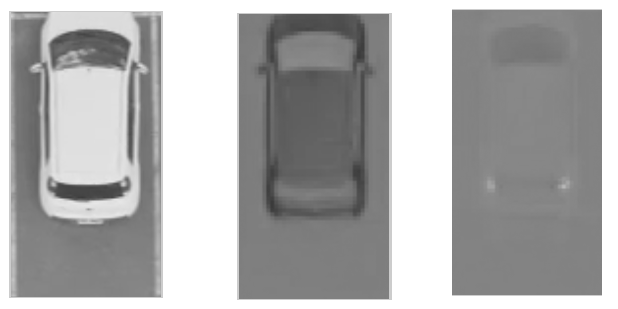
\includegraphics[width=.8\linewidth]{exemploYCbCrFinal}
	\caption{}
	\label{fig:Espacos:sub:YCbCr}
\end{subfigure}
\caption{(a) Uma imagem e cada um de seus canais RGB ordenados da esquerda para a direita e (b) os canais YCbCr da imagem ordenados da esquerda para a direita.}
\label{fig:Espacos}
\end{figure}

\subsection{Descritores de textura}\label{sec:descritores}

Descritores de textura são algoritmos que procuram fazer o que o olho humano faz com facilidade: distinguir entre tipos diferentes de objetos apenas por algumas de suas características visuais. Estes algoritmos são utilizados quando a abordagem de processamento \textit{pixel-a-pixel} se mostra insuficiente. Eles observam e analisam características pertinentes a imagem inteira e são capazes de identificar diferenças mais sutis entre imagens diferentes. Existem diversas técnicas de descrição de textura que são utilizadas com sucesso em aplicações de processamento de imagem. Para esse trabalho, a técnica escolhida foi a conhecida como GLCM(\textit{gray-level co-ocurrence matrix}) descrita na seção \ref{sec:GLCM}, por ter execução rápida e ser invariante quanto a escala de cinza.

\subsection{GLCM}\label{sec:GLCM}

GLCM, ou matriz de co-ocorrência de nível de cinza, é uma técnica de descrição de textura que visa extrair medidas estatíticas da imagem sendo analisada. Para tanto, é criada uma matriz quadrada de tamanho $MxM$ onde M é a quantidade de níveis de cinza possíveis na imagem em questão. Essa matriz armazena a probabilidade de dois \textit{pixels} se relacionarem através de uma certa relação espacial\cite{GLCM}. 

Para esse trabalho, a relação observada é a da vizinhança entre dois \textit{pixels}, sempre analisando o valor a direita de um determinado \textit{pixel} da imagem. Os 255 valores de intensidade possíveis são divididos em 8 níveis. Cada elemento $P_{i,j}$ na GLCM $G$ conta a quantidade de vezes que um \textit{pixel} com valor de intensidade no nível $j$ apareceu à direita de um \textit{pixel} com valor no nível $i$. A figura \ref{fig:GLCM} exemplifica a criação da GLCM a partir de uma imagem com 8 níveis possíveis.

\begin{figure}
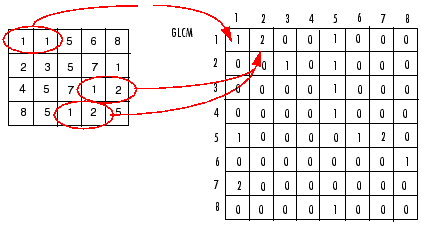
\includegraphics[width=8cm]{GLCM} 
\centering
\caption{Exemplo da elaboração da GLCM. Extraída de https://www.mathworks.com/help/images/ref/graycomatrix.html}
\label{fig:GLCM}
\end{figure}

Uma vez criada a imagem, diversas medidas podem ser tiradas. Para esse trabalho são extraídas 4 características definidas abaixo. Nas equações apresentadas $P_{(i,j)}$ representa o valor do elemento na posição $(i,j)$ da GLCM, $\mu_i$ e $\mu_j$ representam a média dos valores de $i$ e $j$ respectivamente e $\sigma_i$ e $\sigma_j$ os desvios padrão destes valores.

\begin{itemize}

\item Contraste: mede o contraste entre um \textit{pixel} e seu vizinho na imagem. Deve ser 0 para uma imagem completamente homogênea. Definido por:
	\begin{equation}
		C = \sum_{i,j} (i-j)^{2}P_{(i,j)}
	\end{equation}
	
\item Correlação: mede a taxa de correlação de um \textit{pixel} e seu vizinho na imagem inteira. Definida por:
	\begin{equation}
		Co = \sum_{i,j} \frac{(i - \mu_i)(j - \mu_j)P_{(i,j)}}{\sigma_i\sigma_j}
	\end{equation}
	
\item Energia: soma do quadrado dos elementos da imagem. Definida por:
	\begin{equation}
		E = \sum_{i,j} P_{(i,j)}^{2}
	\end{equation}
	
\item Homogeneidade: mede a proximidade da distribuição dos elementos à diagonal da matriz. Definida por:
	\begin{equation}
		H = \sum_{i,j} \frac{P_{(i,j)}}{1+|i-j|}
	\end{equation}
\end{itemize}






